% !TeX encoding = utf8
% !TeX program = pdflatex
% !TeXpellcheck = it_IT

\documentclass[a4paper,11pt,oneside]{article} 

\usepackage{relazioni}
\usepackage{imakeidx}
\usepackage{colortbl}
\usepackage{booktabs}
\usepackage{blindtext}
\usepackage{titletoc}
\usepackage{hyperref}
\usepackage{graphicx}
\usepackage{subcaption}
\usepackage{wrapfig}
\usepackage{geometry}
\usepackage{array}
\usepackage[export]{adjustbox}
\usepackage{multirow}
\usepackage{multicol}

\usepackage{colortbl}


\graphicspath{{Figure/}}

\begin{document}
\input{Front-matter/Frontespizio}

\tableofcontents
\addtocontents{toc}{~\hfill{Pagina}\par}
\contentsmargin{6em}
\dottedcontents{section}[1em]{\bigskip}{2em}{1pc}
\dottedcontents{subsection}[3em]{\smallskip}{3em}{1pc}
\dottedcontents{subsubsection}[5em]{\smallskip}{4em}{1pc}


\newpage

\section{Obiettivo}
L'obiettivo dell'esperienza è la verifica del comportamento elastico di un filo metallico, la stima del suo coefficiente elastico $K$ e del relativo modulo di Young $E$, dopo aver definito il miglior protocollo di misura.

\section{Apparato sperimentale}\label{section:apparato}

\begin{figure}[h!]
    \centering
    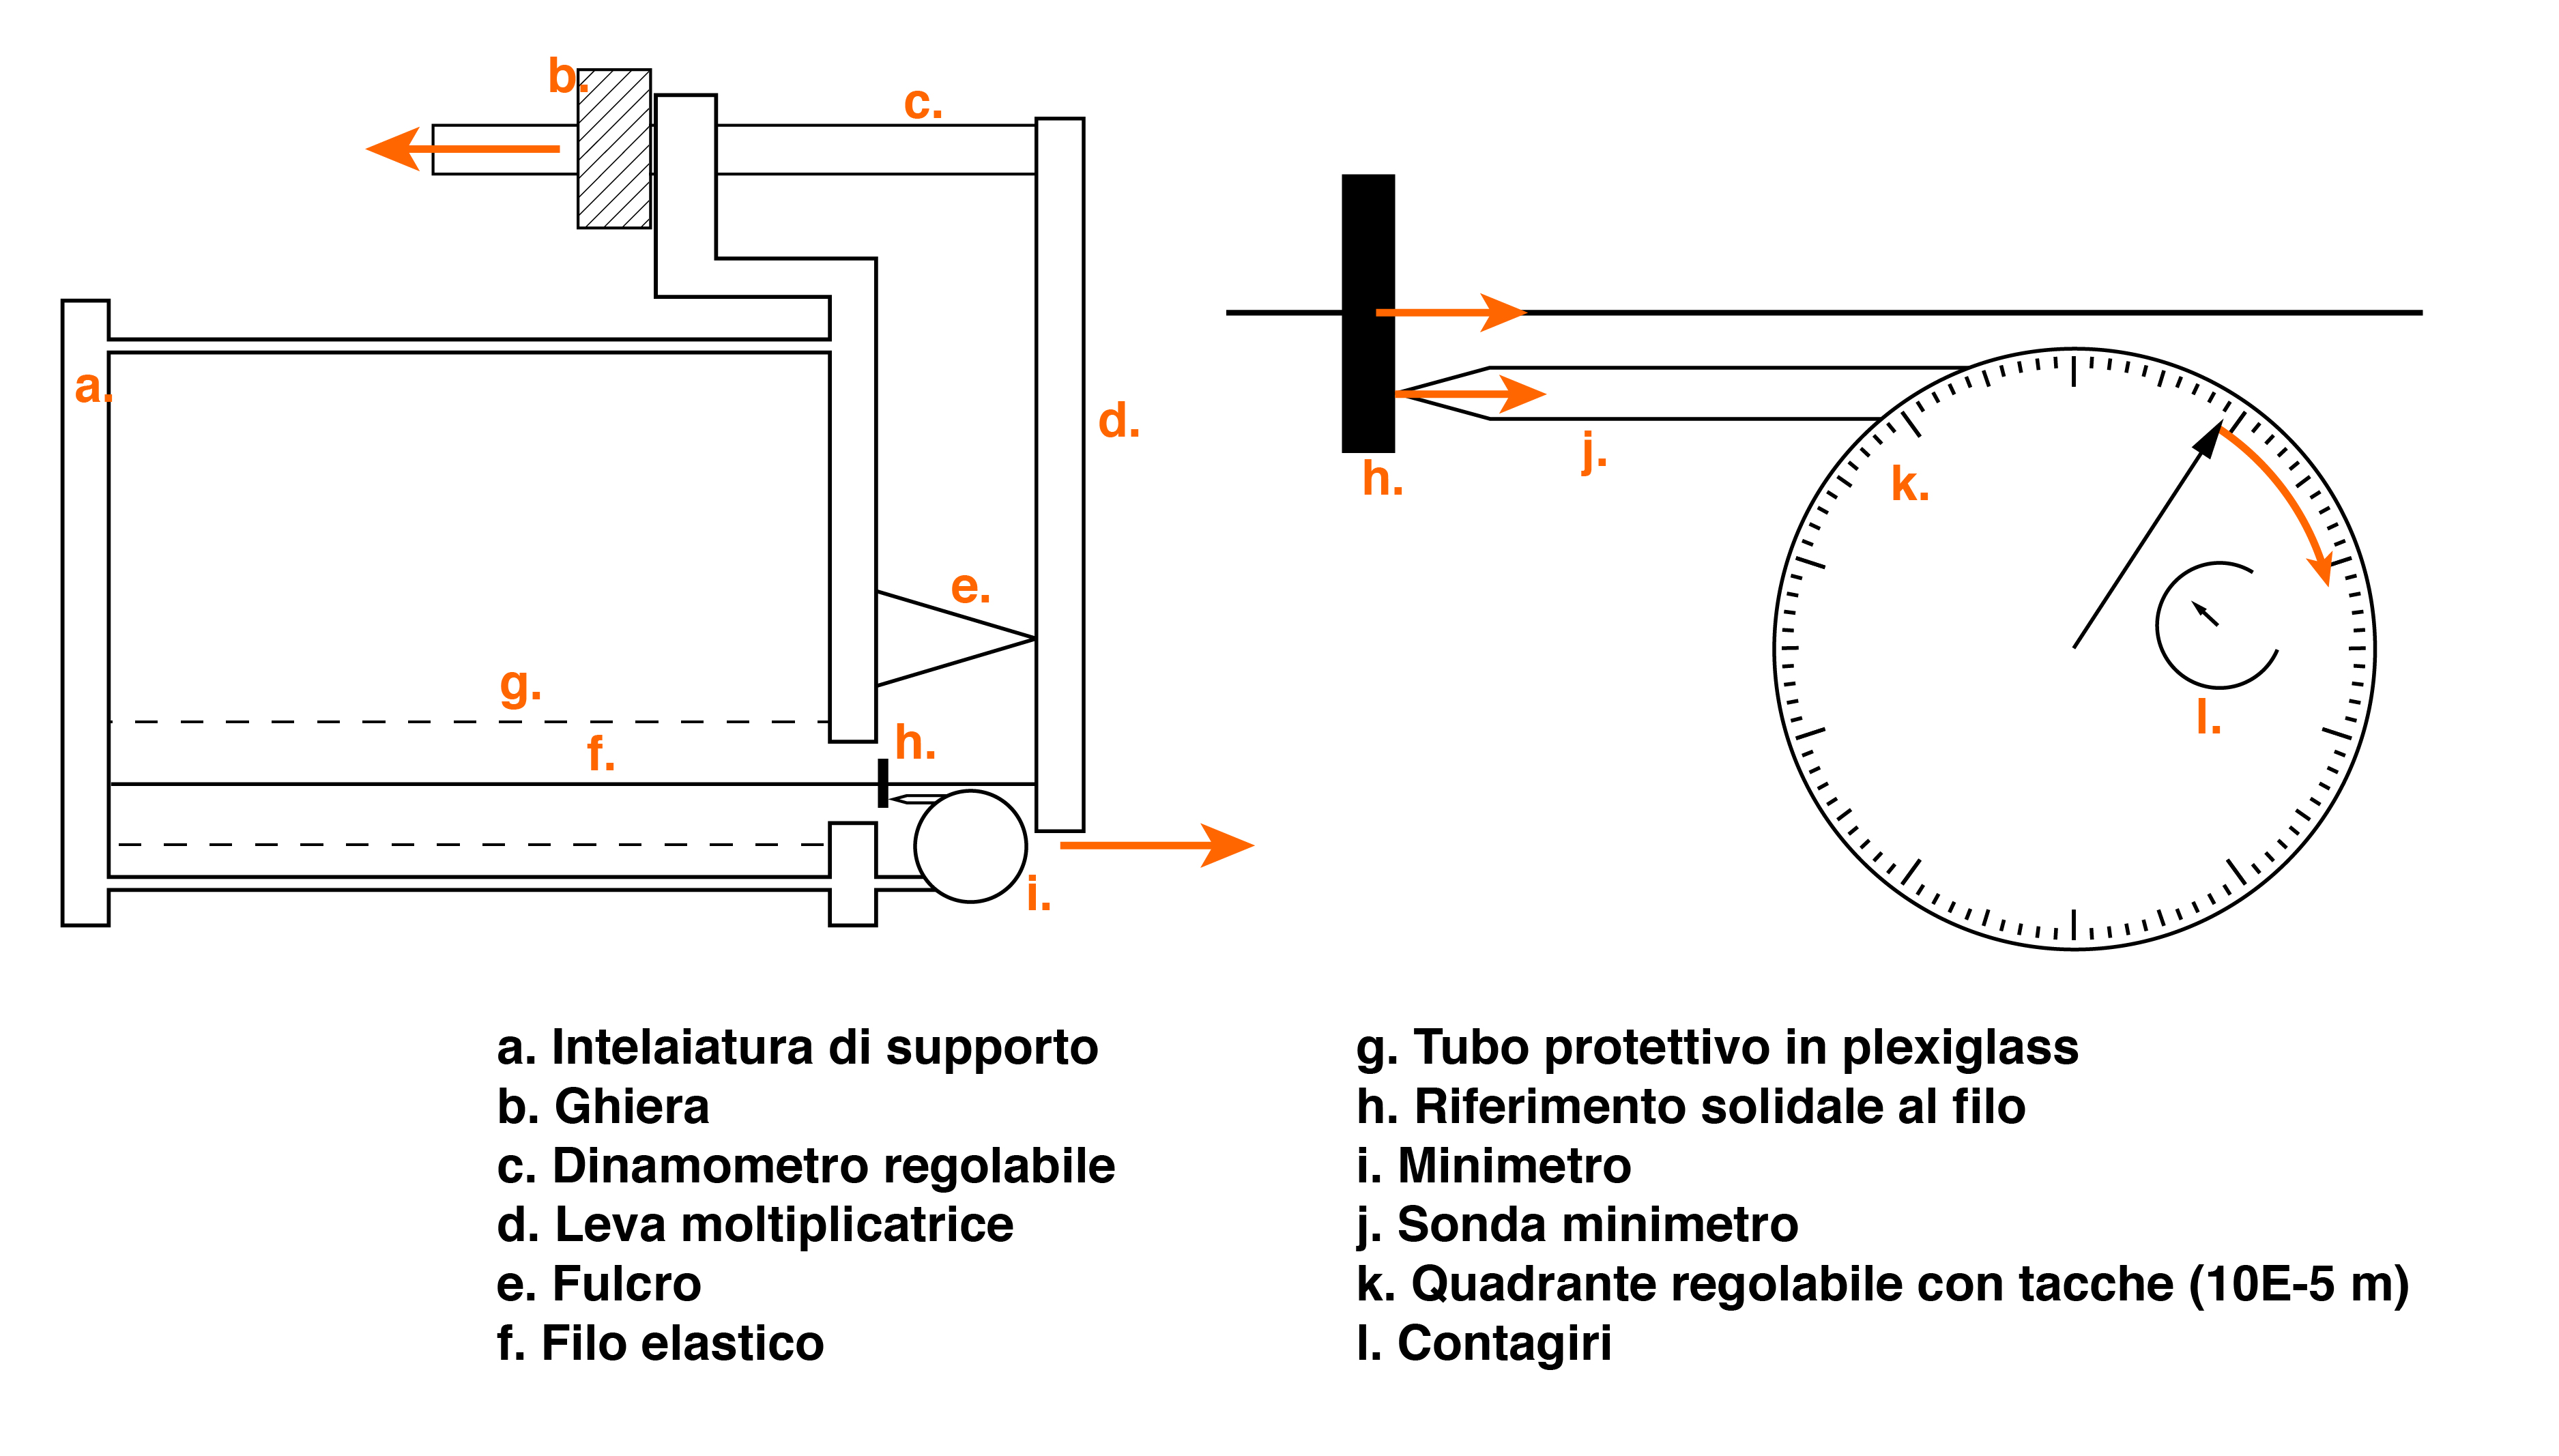
\includegraphics[width=12.5cm]{ApparatoSperimentale.jpg}
    \caption{Diagramma composizione apparato sperimentale}
    \label{fig:apparato_sperimentale}
\end{figure}
L'apparato sperimentale risulta così composto:
\begin{enumerate}
    \item Un cilindro metallico posto internamente ad un tubo protettivo a tutela di perturbazioni esterne. Lo stesso ha un'estremità fissata in maniera solidale alla struttura di supporto e nella parte finale presenta un disco forato, al fine di valutarne l'allungamento.
    \item Un minimetro a quadrante regolabile con sensibilità $S=\num{1e5} \si{m^{-1}}$ con sonda appoggiata al riferimento. E' presente inoltre un contatore interno al quadrante del minimetro che tiene conto dei giri completi compiuti dalla lancetta.
    \item Un dinamometro regolabile tramite una ghiera che, ruotando, varia la forza applicata al filo. L'unità di misura utilizzata è grammi peso, avente la più piccola tacca di lettura pari $\SI{100}{gp}$
    \item Una leva collegata al filo metallico e al dinamometro utilizzata per quadruplicare la forza esercitata dal dinamometro.
\end{enumerate}
Nel complesso sono stati impiegati 11 estensimetri diversi, dei quali vengono riassunte le caratteristiche nella Tabella \ref{tab:caratteristiche_estensimetri}.

\begin{table}
	\centering
	\begin{tabular}{lccc}
		    Materiale & \#& \multicolumn{1}{l}{Lunghezza}        & \multicolumn{1}{l}{Diametro}\\ 
		    &&$[\si{mm}] \pm\SI{2}{mm}$&$[\si{mm}] \pm\SI{1}{\percent}$\\
		\hline
\multirow{9}{*}{Acciaio} & {\cellcolor[rgb]{0.753,0.753,0.753}}1  & {\cellcolor[rgb]{0.753,0.753,0.753}}950  & {\cellcolor[rgb]{0.753,0.753,0.753}}0.33   \\
& 2 & 950 & 0.356  \\
& {\cellcolor[rgb]{0.753,0.753,0.753}}3  & {\cellcolor[rgb]{0.753,0.753,0.753}}950  & {\cellcolor[rgb]{0.753,0.753,0.753}}0.381  \\
& 4 & 950 & 0.305  \\ & {\cellcolor[rgb]{0.753,0.753,0.753}}5  & {\cellcolor[rgb]{0.753,0.753,0.753}}950  & {\cellcolor[rgb]{0.753,0.753,0.753}}0.3    \\
& 6 & 950 & 0.4                                        \\
& {\cellcolor[rgb]{0.753,0.753,0.753}}7  & {\cellcolor[rgb]{0.753,0.753,0.753}}950  & {\cellcolor[rgb]{0.753,0.753,0.753}}0.279  \\
& 8 & 600 & 0.279                                      \\
& {\cellcolor[rgb]{0.753,0.753,0.753}}9  & {\cellcolor[rgb]{0.753,0.753,0.753}}800  & {\cellcolor[rgb]{0.753,0.753,0.753}}0.279  \\
& 10 & 700 & 0.279                                      \\

Tungsteno & {\cellcolor[rgb]{0.753,0.753,0.753}}11 &{\cellcolor[rgb]{0.753,0.753,0.753}} 1000 &{\cellcolor[rgb]{0.753,0.753,0.753}} 0.25\\
Ottone                   & 12 & 1000 & 0.5   
\end{tabular}
	\caption{Estensimetri impiegati}
	\label{tab:caratteristiche_estensimetri}
\end{table}



\section{Metodi acquisizione dati}
Si specifica che i dati relativi alla prima parte sono stati trascritti da registrazioni video dell'apparato sperimentale. I dati invece impiegati nell'analisi sistematica dei vari estensimetri sono invece stati direttamente forniti in tabelle.\\
In questa sezione vengono esposti i due diversi metodi impiegati per raccogliere i dati dagli estensimetri.
\subsection{Primo metodo - Allungamento e Accorciamento}%aumento di 100 in 100
Come operazione preliminare si è agito sulla ghiera dell'estensimetro, manovrandola in modo tale che segnasse una tensione $F_{letta}=\SI{200}{gp}$ così da mettere in tensione il filo di metallo analizzato. Si è poi sollecitata delicatamente la manopola della sonda del minimetro così da eliminare l'eventuale contributo di giochi meccanici ed infine si è impostata la ghiera del minimetro in modo che lo zero del quadrante coincidesse con la posizione della lancetta maggiore. Dopo aver annotato il valore letto sul minimetro, tendendo in considerazione che una rotazione completa della lancetta corrisponde una variazione di lunghezza pari a $\num{1} \si{mm}$, si è manovrata la ghiera del dinamometro portandola alla tacca successiva, ovvero aumentando la forza letta di $\SI{100}{gp}$. Avendo cura di non oltrepassare la tacca e di smuovere la manopola della sonda di volta in volta, si sono annotati tutti i valori segnati dal minimetro. La ghiera è stata manovrata fino ad arrivare ad una forza letta di $\SI{1200}{gp}$. A tal punto si è diminuita la tensione esercitata dal dinamometro, variando sempre la $F_{letta}$ di $\SI{100}{gp}$ in $\SI{100}{gp}$, e annotando i valori del minimetro.\\

\subsection{Secondo metodo - Misure ripetute}%video 400 -1000
Riportato l'estensimetro con il dinamometro a $\SI{200}{gp}$ si sono eseguite misure ripetute. La procedura è consistita nel portare il dinamometro ad esercitare una tensione letta di $\SI{400}{gp}$, dapprima aumentandola a partire da $\SI{200}{gp}$, poi diminuendola a partire da $\SI{600}{gp}$. È stata prestata la massima attenzione nel non oltrepassare la tacca di $\SI{400}{gp}$. %Questa accortezza ha permesso di salvaguardare le misure da eventuali errori derivanti da fenomeni di isteresi meccanica.
Il procedimento è stato effettuato 18 volte in corrispondenza della tacca $\SI{400}{gp}$ per poi ripetere la presa dati in corrispondenza della tacca di $\SI{1000}{gp}$, variando in accorciamento fino a $\SI{800}{gp}$ e in allungamento fino a $\SI{1200}{gp}$.\\
E' opportuno precisare che l'analisi dei video è stata compiuta singolarmente: ogni operatore ha trascritto la lettura del minimetro corrispondente ad ogni misurazione, in modo da avere un campione più significativo e compiere una analisi statistica più accurata.

\section{Analisi dati}

\subsection{Prima parte - Verifica dell'elasticità meccanica e definizione miglior protocollo di misura}
Sono stati impiegati diversi metodi per il calcolo del coefficiente elastico del filo a seconda del metodo di raccolta dati.\\
Nella prima parte l'analisi si è svolta esclusivamente sull'estensimetro numero 10 riportato in Tabella \ref{tab: DEGLI ESTENSIMETRI}. Nella seconda parte invece si è svolta un'analisi sistematica su tutti gli estensimetri in acciaio.
\subsubsection*{Primo Metodo - Misure in allungamento e accorciamento}
Per la prima acquisizione dati si è scelto di calcolare separatamente due diversi valori di K, mantenendo separati i dati raccolti quando il filo veniva allungato e quando il filo veniva accorciato. Si è utilizzato il metodo del minimo $\chi^2$ al fine di calcolare il coefficiente elastico, sfruttando la relazione lineare che lega l'allungamento o l'accorciamento del filo con la forza applicata per metterlo in tensione. La relazione è la seguente e prende il nome di legge di Hooke:
\begin{equation*}
       \left | x_i - x_0  \right |  = k \cdot  \left | \Delta F \right |
\end{equation*}
Partendo dai dati raccolti da ciascun operatore è stata calcolata la media delle acquisizioni relative alla stessa misurazione ed in seguito sono stati calcolati gli errori ad essa associati. Per il calcolo di quest'ultimo, al fine di non sottostimare l'errore si è  valutato opportunamente sia la deviazione standard della media e sia l' errore derivante dalla distribuzione uniforme, in modo da utilizzare la stima dell'errore più appropriata. Accadeva infatti che le misure dei tre operatori coincidessero e pertanto la $\overline{\sigma}$ fosse nulla. Per evitare un errore nullo si è tenuto in considerazione l'errore derivante dalla distribuzione uniforme con ptl pari a 10 micron e coefficiente di affidabilità pari a 10.
%ABBIAMO FORSE SOTTOSTIMATO L'ERRORE DUNQUE CAMBIARE QUESTA PARTE
Analogamente per l'incertezza sulla forza applicata si è usata la distribuzione triangolare considerando come ptl il doppio dello spessore della tacca incisa.
Per l'utilizzo del $\chi^2$ si sono confrontati i due errori e si è scelto strategicamente, in quando minore rispetto all'errore su $\Delta x$, di trascurare l'errore sulla forza e di utilizzarla come grandezza sull'asse delle ascisse.\\
Si sono ottenuti i valori dei coefficienti angolari K e delle intercette con l'asse delle ordinate per le misure in allungamento e in accorciamento ed è stato associato ad esse l'errore derivante dal metodo del minimo $\chi^2$, come descrivono le formule \ref{equation:err_chi_quadro}.\\
E' stata calcolata la compatibilità tra i due valori di K ottenuti e tra le due intercette. Si è fatto riferimento alle seguenti per valutare $\lambda$ e la sua bontà:
\begin{equation*}%Comp
    \label{eq:cases}
    \begin{cases}
    0<\lambda\leq 1, & \text{Ottima}\\
    1<\lambda\leq2, & \text{Discreta}\\
    2<\lambda\leq3, & \text{Pessima}\\
    3<\lambda, & \text{Non compatibile}\\
    \end{cases}
\end{equation*}
Successivamente gli errori sui coefficienti angolari e sulle intercette sono stati valutati nuovamente prendendo invece in considerazione la sigma a posteriori derivante dal chi quadro. Analogamente a quanto fatto precedentemente, si è calcolata nuovamente la compatibilità.\\
Viene riportato in Figura \ref{fig:GRAFICO ALL ACC} il grafico dell'andamento delle misure con le relative interpolazioni.
Per dare infine una stima del coefficiente K si è eseguita la media ponderata fra il $K_{all}$ e il $K_{acc}$ precedentemente ottenuti mediante la Formula \ref{equation:NOMEFORMULA PROPAGAZIONE}. Analogo procedimento è stato ripetuto per i valori delle intercette in allungamento ed in accorciamento. Vengono riportati in Tabella \ref{tab: TABELLA K E COMPATIBIITÀ}.

\subsubsection*{Secondo Metodo - Misure ripetute}
Per il calcolo di K tramite misure ripetute sono stati utilizzati due procedimenti differenti.\\
Nel primo caso, al fine di apprezzare eventuali evidenze sperimentali celate dal metodo precedente, si è optato per il calcolo del coefficiente di elasticità direttamente mediante la legge di Hooke, calcolando $\Delta x$ medi per ogni sottocampione di misurazioni.\\ 

In primo luogo si è proceduto con il calcolo delle medie delle misurazioni di ogni operatore, nello specifico per le misure di allungamento e accorciamento per $F_{letta}$ pari a $\SI{400}gp$ e $\SI{1000}gp$ distinguendo se si fosse raggiunta la tacca prescelta aumentando o diminuendo la forza dal dinamometro. Di ogni campione $F_{400, all}$, $F_{400, acc}$, $F_{10000, all}$ e $F_{10000, acc}$ si è calcolata la media, associandovi come errore la relativa $\overline{\sigma_x}$.\\
Per ogni campione, utilizzando la legge di Hooke, si sono ottenuti 4 valori differenti di coefficiente elastico ottenendo $K_{400, all}$, $K_{400, acc}$, $K_{1000, all}$ e $K_{1000, all}$ impiegando come $\Delta x$ quelli appena ricavati e come $\Delta F$ la differenza tra $\SI{400}{gp} / \SI{1000}{gp} - \SI{200}{gp}$ . L'errore di ogni K è stato calcolato utilizzando la propagazione degli errori tramite la seguente:
\begin{equation*}
   \sigma_k=\sqrt{\left ( \frac{\partial k }{\partial F } \right )^{2}\sigma_F^2 \cdot \left ( \frac{\partial k }{\partial \Delta_x } \right )^{2}{\sigma_\Delta_x}^2} 
\end{equation*}
E' stata poi effettuata la media ponderata dei due coefficienti elastici "in allungamento" ($K_{400, all}$ e $K_{1000, all}$) e dei due "in accorciamento" ($K_{400, acc}$ e $K_{1000, acc}$) sempre associando il relativo errore. Infine per restituire un valore unico di K si è nuovamente calcolata la media ponderata fra questi due ultimi valori, associandovi l'errore. Infine si è valutata la compatibilità fra ${\langle K \rangle}_{all}$ e ${\langle K \rangle}_{acc}$. Tutti i dati citati sono riportati in Tabella \ref{tab: TABELLA DATI K SECONDO METODO con COMPATIBILITÀ}.\\

Il secondo metodo per le misure ripetute è consistito nel calcolo del Chiquadro su tutte le misure ottenute a 400gp e 10000gp con l'accortezza di distinguere i dati presi in allungamento ed in accorciamento. Operando secondo questo schema si sono ottenute due rette di interpolazione, una per i dati delle misure "in allungamento" ed una per quelli "in accorciamento". I due coefficienti angolari rappresentano i coefficienti rispettivamente di allungamento e di accorciamento e da essi si è ricavata la media ponderata, rappresentativa della costante elastica dell'estensimetro in esame e la compatibilità fra ${K}_{acc}$ e ${K}_{all}$. Vengono riportati i dati qui citati in Tabella \ref{tab: TABELLA SECONDO METODO SECONDA ACQUISIZIONE}

%MISURAZIONI DI 100 IN 100
% -CHI QUADRO
% ////-CAMPIONI DI K (NON SONO STATI FATTI)
%CONSECUTIVE
% -
%PROTOCOLLO DI MISURA
% - I GRAFICI CHE SERVON PER DIMOSTRARE POI< PARLANE E METTILI

\subsection{Seconda parte - Stima di $K$ e di $E$ per gli estensimetri}
Dai dati forniti, si sono calcolati i $\Delta x$ come differenza tra le misure $x_n$ e $x_0$ separatamente per allungamento e accorciamento, corrispondenti ad una $\Delta F_{app} = F_{x, app} - F_{0, app}$. Ai $\Delta x$ è stato associato l'errore calcolato con la propagazione degli errori casuali in cui $\sigma_{F}$ deriva dalla distribuzione uniforme, ponendo come più piccola tacca di misura $\SI{5}{micron}$ e coefficiente di affidabilità 1.
Similmente a quanto descritto nella prima acquisizione, dopo una rappresentazione grafica dei dati, si sono calcolati i $K_{all}$ e i $K_{acc}$ ed i relativi errori per tutti gli estensimetri dotati di filo in acciaio tramite il metodo del $\chi^2$. Per associare la giusta incertezza ai parametri del fit lineare si sono confrontati gli errori $\sigma_{\Delta x}$ e $\sigma_{\Delta x, posteriori}$. Per evitare una possibile sottostima dell'errore nell eordinate è stato considerato il contributo maggiore. Si è poi calcolata la media ponderata tra i $K_{all}$ e $K_{acc}$ come stima del ${\langle K\rangle }\pm \sigma_{{\langle K\rangle }}$ e la compatibilità fra $K_all$ e $K_acc$ e fra $Intercetta_all$ e $Intercetta_acc$ per ciascun estensimetro come viene esposto nella Tabella \ref{tab: MEGA TABELLA CON TUTTI I K ALL E ACC DI TUTTI EST CON MEDI EPONDERATE E COMPATIBILIT}

\begin{figure}[H]
    \centering
    \subfloat[Estensimetro 1]{
        \label{fig:1_estensimetro}
        \includegraphics[width=7.5cm]{1_estensimetro.png}
    }
    \subfloat[Estensimetro 2]{
        \label{fig:2_estensimetro}
        \includegraphics[width=7.5cm]{2_estensimetro.png}
    }
    \newline
    \subfloat[Estensimetro 3]{
        \label{fig:3_estensimetro}
        \includegraphics[width=7.5cm]{3_estensimetro.png}
    }
    \subfloat[Estensimetro 4]{
        \label{fig:4_estensimetro}
        \includegraphics[width=7.5cm]{4_estensimetro.png}
    }
    \newline
    \subfloat[Estensimetro 5]{
        \label{fig:5_estensimetro}
        \includegraphics[width=7.5cm]{5_estensimetro.png}
    }
    \subfloat[Estensimetro 6]{
        \label{fig:6_estensimetro}
        \includegraphics[width=7.5cm]{6_estensimetro.png}
    }
    \newline
    \subfloat[Estensimetro 7]{
        \label{fig:7_estensimetro}
        \includegraphics[width=7.5cm]{7_estensimetro.png}
    }
    \subfloat[Estensimetro 8]{
        \label{fig:8_estensimetro}
        \includegraphics[width=7.5cm]{8_estensimetro.png}
    }
    
\end{figure}
\begin{figure}[h!]
    \centering
    \subfloat[Estensimetro 9]{
        \label{fig:9_estensimetro}
        \includegraphics[width=7.5cm]{9_estensimetro.png}
    }
\end{figure}

%TRE METODI PER IL MODULO DI YOUNG
\newpage

\section{Discussione dei risultati}
% - ERRORE DI ISTERESTI DIMOSTRATO CON CHI QUADRO 
% - ERRORE DI DESALVADOR

\subsection{Prima esperienza}
\subsection{Seconda esperienza}

\section{Margini di miglioramento}

\section{Conclusione}

\section{Appendice}

\subsection{Formulario}
\textbf{Media, deviazione standard, deviazione standard della media}
\begin{align*}
   % \begin{aligned}
        \overline{x}&=\sum\limits_{i=1}^{N} \frac{x_{i}}{N}&
        \sigma&=\sqrt{\frac{\sum\limits_{i=1}^{N} (x_{i}-\overline{x})}{N-1}}&
        \sigma_{\overline{x}}&=\frac{\sigma}{\sqrt{N}}
   % \end{aligned}
\end{align*}\\

\textbf{Media Ponderata}
\begin{equation*}\
    x_i=\frac{\sum_{i=1}^{N}\frac{x_i}{\sigma_{x_i}}}{\sum_{i=1}^{N}\frac{1}{\sigma_{x_i}}} \label{eq:media_ponderata}
\end{equation*}

\textbf{Errore Media Ponderata}
\begin{equation*}
     \sigma_{x_i}=\sqrt{\frac{1}{\sum_{i=1}^{N}\frac{1}{\sigma_{i}^{2}}}}\label{eq:errore_media_pond}
\end{equation*}

\textbf{Formule per il ${\chi}^2$}
\begin{equation*}
        \begin{cases}
    a=&\frac{1}{\Delta}[(\sum\limits_{i=1}^{N}{x_{i}^{2}})\cdot(\sum\limits_{i=1}^{N}{y_{i}})-(\sum\limits_{i=1}^{N}{x_{i}})\cdot(\sum\limits_{i=1}^{N}{x_{i}y_{i}})] \\ 
    b=&\frac{1}{\Delta }\cdot \left [N\cdot \left ( \sum\limits_{i=1}^{N}x_i y_i \right )-\left ( \sum\limits_{i=1}^{N}x_i \right )\cdot \left ( \sum\limits_{i=1}^{N}y_i \right )  \right ]\\
    \Delta=& N\cdot \sum\limits_{i=1}^{N} x_i^{2} - \left ( \sum\limits_{i=1}^{N}x_i \right )^{2}\\
    \end{cases}
\end{equation*}
\begin{equation*}
    \begin{cases}
    \sigma_{a}=&\sigma_{y}\cdot\sqrt{\frac{\sum_{i=1}^{N}{x_{i}^{2}}}{\Delta}} \\
    \sigma_{b}=&\sigma_y\cdot \sqrt{\frac{N}{\Delta }}\\
    \end{cases}
    \label{equation:err_chi_quadro}
\end{equation*}
\\
\textbf{Formula di propagazione degli errori casuali}\\

Sia z=($x_1$,...;$x_N$) funzione di N variabili casuali $x_1$,...,$x_N$ e sia ${x_i^\ast}$=($x_1^\ast$,...,$x_N^{\ast}$) l'insieme di tutti i valori veri associati a tali variabili, si ha 

\begin{equation*}
    \sigma_z^{2}\approx  \sum_{i=j=1}^{N}\left ( \frac{\partial z}{\partial x_i}\Big|_{x_i^{\ast}} \right )^{2}\cdot\sigma_{x_i}^{2} +\sum_{i=1,j=1,i\neq j}^{N}\left (\frac{\partial z }{\partial x_i}\Big|_{x_i^{\ast}} \right ) \cdot \left ( \frac{\partial z}{\partial x_j} \Big|_{x_j^{\ast}} \right )\cdot cov(x_i,x_j)\label{eq:prop_errori}
\end{equation*}
E' stato utilizzato il simbolo $\approx$ in quanto si è scelto di troncare al primo termine lo sviluppo in serie di Taylor.\\


\textbf{Formula calcolo compatibilità}\\
\begin{equation*}
    \lambda=\frac{\left|a-b\right|}{\sqrt{\sigma^{2}_{a}+\sigma^{2}_{b}}}
\end{equation*}\\

\subsection{Codice sorgente}
\subsection{Dati Grezzi}
\subsubsection{Prima Parte}
\subsubsection{Seconda Parte}

\end{document}*
